
\documentclass{beamer}

\usepackage{algpseudocode, color, colortbl, listings, MnSymbol}

\usepackage{hyperref}
\hypersetup{
    colorlinks=true,
    urlcolor=blue,
}

\usepackage{tikz, xcolor}

\usetheme{Montpellier}
\usecolortheme{rose}

% page numbers, from
% https://tex.stackexchange.com/questions/137022/how-to-insert-page-number-in-beamer-navigation-symbols
\expandafter\def\expandafter\insertshorttitle\expandafter{%
  \insertshorttitle\hfill%
  \insertframenumber\,/\,\inserttotalframenumber}

\definecolor{Gray}{gray}{0.8}
\newcolumntype{g}{>{\columncolor{Gray}}c}

\newcommand{\stanza}{ \\~\ }

\title{14. Computational Geometry Introduction}
\subtitle{CPSC 535}
\author{Kevin A. Wortman}
\institute{ 
\includegraphics[height=2cm]{csuf-logo-cmyk} }
\date{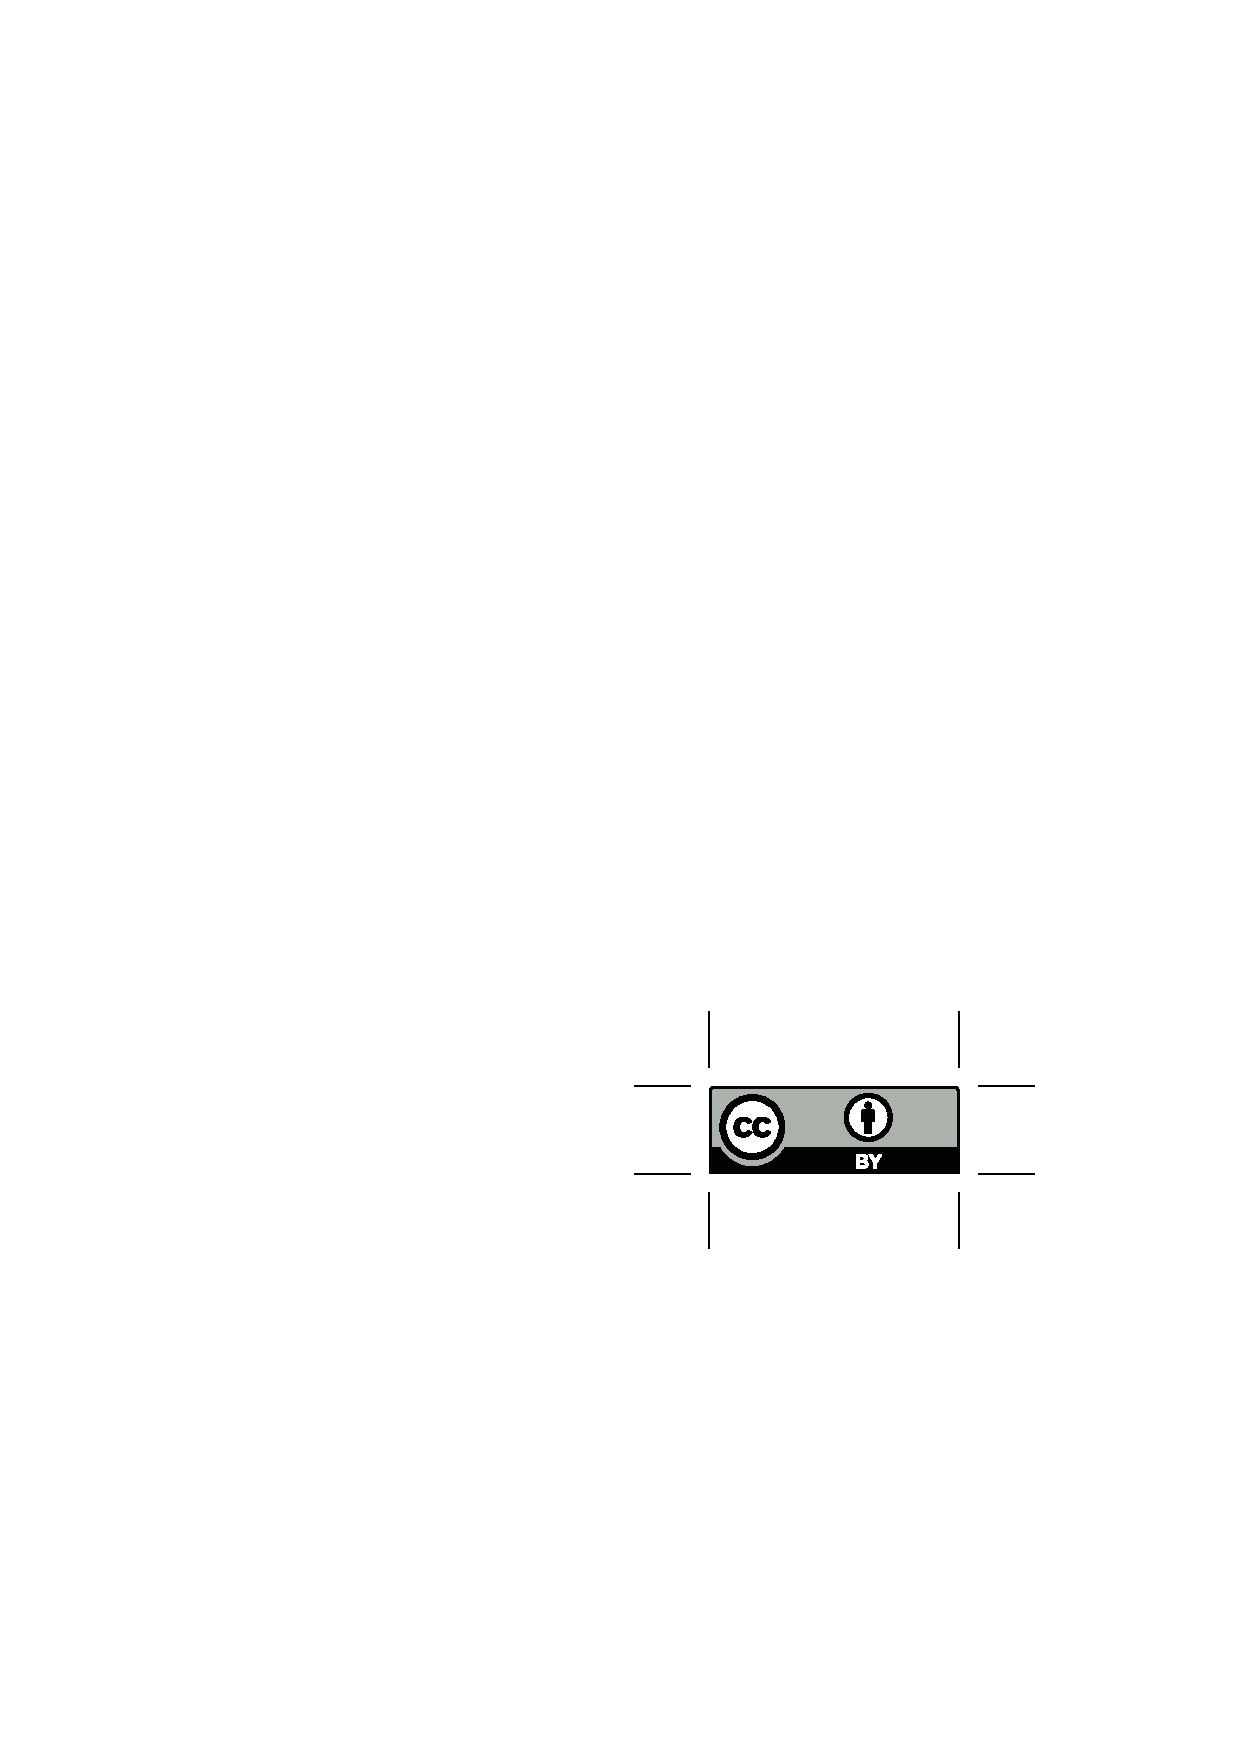
\includegraphics[height=14pt]{by} \\

{\tiny
This work is licensed under a
\href{http://creativecommons.org/licenses/by/4.0/}{Creative Commons Attribution 4.0 International License}.
}}

\begin{document}

\begin{frame}
  \titlepage
\end{frame}


\begin{frame} \frametitle{Big Idea: Problem Duality}
  \textbf{problem duality:} when the input/output mathematical definition of a
  problem can be interpreted by humans in two (or more) very different ways
  \begin{itemize}
    \item one algorithm can solve multiple problems with different ``stories''
    \item algorithms, computers, don't actually care what data values mean
    \item turns out max-flow and min-cut are two different stories for the same problem
    \item max-flow and min-cut are the \emph{dual of each other}
  \end{itemize}
  \end{frame}
  
  \begin{frame} \frametitle{Duality Example}
  \textbf{maximum $y$ coordinate} \\
  \emph{input: } a set of $(x, y)$ points $S=\{(x, y) \, | \, x, y \in \mathbb{R} \}$ \\
  \emph{output: } the greatest $y$-coordinate in $S$ \stanza
  
  \textbf{highest $y$-intercept point problem} \\
  \emph{input: } a set of $y=mx+b$ lines $L=\{(m, b) \, | \, m, b \in \mathbb{R} \}$ \\
  \emph{output: } the greatest $y$-intercept $b$ in $L$ \stanza
  \end{frame}
  
  \begin{frame} \frametitle{Geometry Sketch}
  \begin{center}
  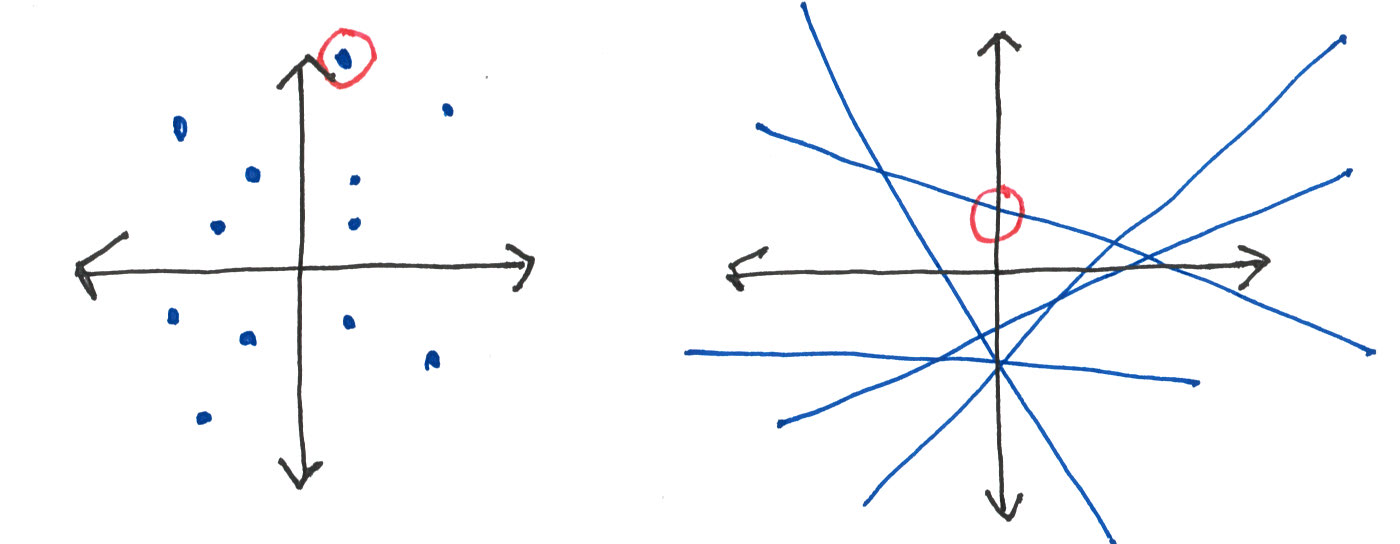
\includegraphics{lines.png}
  \end{center}
  \end{frame}
  
  \begin{frame} \frametitle{}
  C++ functions for these would be declared like:
  \lstinline!double maximum_y_coord(vector<pair<double, double>>& points);!
  \lstinline!double highest_y_intercept(vector<pair<double, double>>& lines);! \stanza
  
  As far as the computer is concerned, these are interchangeable! \stanza
  
  Only the human story differs.
  The
  \textbf{maximum $y$ coordinate}
  and
  \textbf{highest $y$-intercept point problem}
  problems are the dual of each other.
\end{frame}

\begin{frame} \frametitle{Big Idea: Output Sensitive Algorithm}
  \begin{itemize}
    \item \textbf{input sensitive}: time efficiency is a function of the input
      e.g. size $n$, \# edges $m$
    \item \textbf{output sensitive}: efficiency is also a function of the
      \emph{output} size e.g. \# items returned
    \item most relevant when the size of the output could be the
      bottleneck
  \end{itemize}
\end{frame}

\begin{frame} \frametitle{Computational Geometry}
\textbf{computational $X$}: interdisciplinary study of computer science with $X$ \stanza

(computational finance, epidemiology, physics, finance, etc.) \stanza

\emph{computational geometry (CG):} algorithms, data structures, asymptotic analysis, of
geometric objects: points, lines, circles, triangle meshes, etc.
\end{frame}

\begin{frame} \frametitle{Computational Geometry Applications}

Applications of CG:
\begin{itemize}
  \item 3D computer graphics
  \item graphical user interfaces (GUIs)
  \item geographic information systems (GIS), geographic databases
  \item scene reconstruction, self-driving cars (e.g. LIDAR)
  \item business operations research (e.g. linear programming, aircraft control)
  \item manufacturing (e.g. feasibility of assembly, castings)
\end{itemize}
\end{frame}

\begin{frame} \frametitle{Putting the Geo in CG}
Some general algorithms can actually solve geometric problems efficiently, without
any awareness of geometry. \stanza

\begin{columns}
  \begin{column}{0.7 \textwidth}
  \emph{bounding box problem} \\
  \textbf{input}: set of 2D points $P=\{p_1, p_2, \ldots, p_n\}$ \\
  \textbf{output}: points $tl=(x_l, y_t)$ and $rb=(x_r, y_b)$ such that the rectangle
  with top-left corner $tl$ and bottom-right corner $rb$ contains $P$ \stanza
  \end{column}
  \begin{column}{0.3 \textwidth}
    \begin{center}
      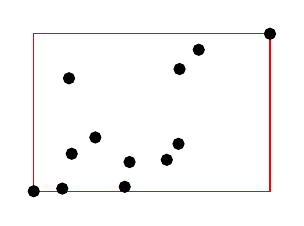
\begin{tikzpicture}
        \draw [color=red] (0, 0) -- (3, 0) -- (3, 2) -- (0, 2) -- (0, 0);
        \foreach \Point in {
          % definining the bounding box
          (0, 0), (3, 2),
          % 10 random points
          (2.0951240918974277, 1.7968031777699034),
          (1.6893802109325138, 0.3988643181954554),
          (0.4478056694086142, 1.434611748573361),
          (1.21650131559343, 0.3708718939225579),
          (0.3622805800271429, 0.03376103132220609),
          (0.48201024301923834, 0.47617070155843133),
          (1.8378918317441353, 0.6021102667795148),
          (0.7819121241895028, 0.6833500815401432),
          (1.155185084745803, 0.05634877501390312),
          (1.8516975398072102, 1.5517971681158893) } {
          \draw [fill=black] \Point circle [radius=2pt];
        }
      \end{tikzpicture}
    \end{center}
  \end{column}
\end{columns}

Na\"{i}ve, optimal algorithm:
$x_l = \min x, y_t = \max y, x_r = \max x, y_b = \min y$;
$\Theta(n)$ time \stanza

Computational geometers are more interested when geometric properties matter.
\end{frame}

\begin{frame} \frametitle{Line Segment Predicates}
We can use arithmetic to answer any of the following predicates (questions)
about points $p_0, p_1, p_2, p_3$ in $\Theta(1)$ time: \stanza
\begin{enumerate}
  \item Is line segment $\overline{p_0 p_1}$ clockwise from $\overline{p_0 p_2}$
    around the common endpoint $p_0$?
  \item If we follow $\overline{p_0 p_1}$ and then $\overline{p_1 p_2}$, do we
    turn right or left?
  \item Do line segments $\overline{p_0 p_1}$ and $\overline{p_2 p_3}$
    intersect? \stanza
\end{enumerate}

$\implies$ We may use any of these in pseudocode.
\end{frame}

\begin{frame} \frametitle{Line Segment Predicates}
  \begin{center}
    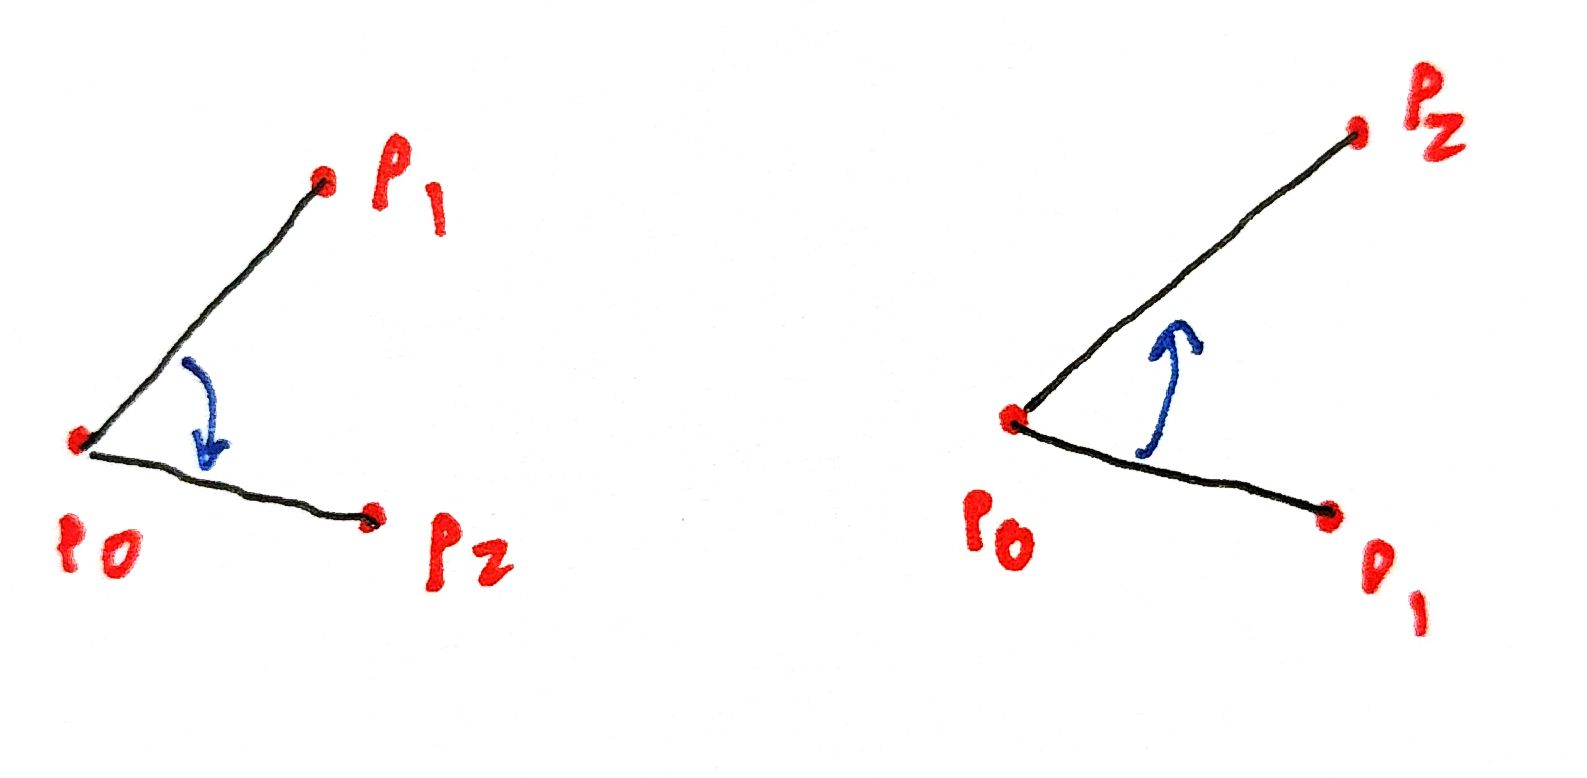
\includegraphics[width=4cm]{segment_clockwise.jpg}
    \hspace{2cm}
    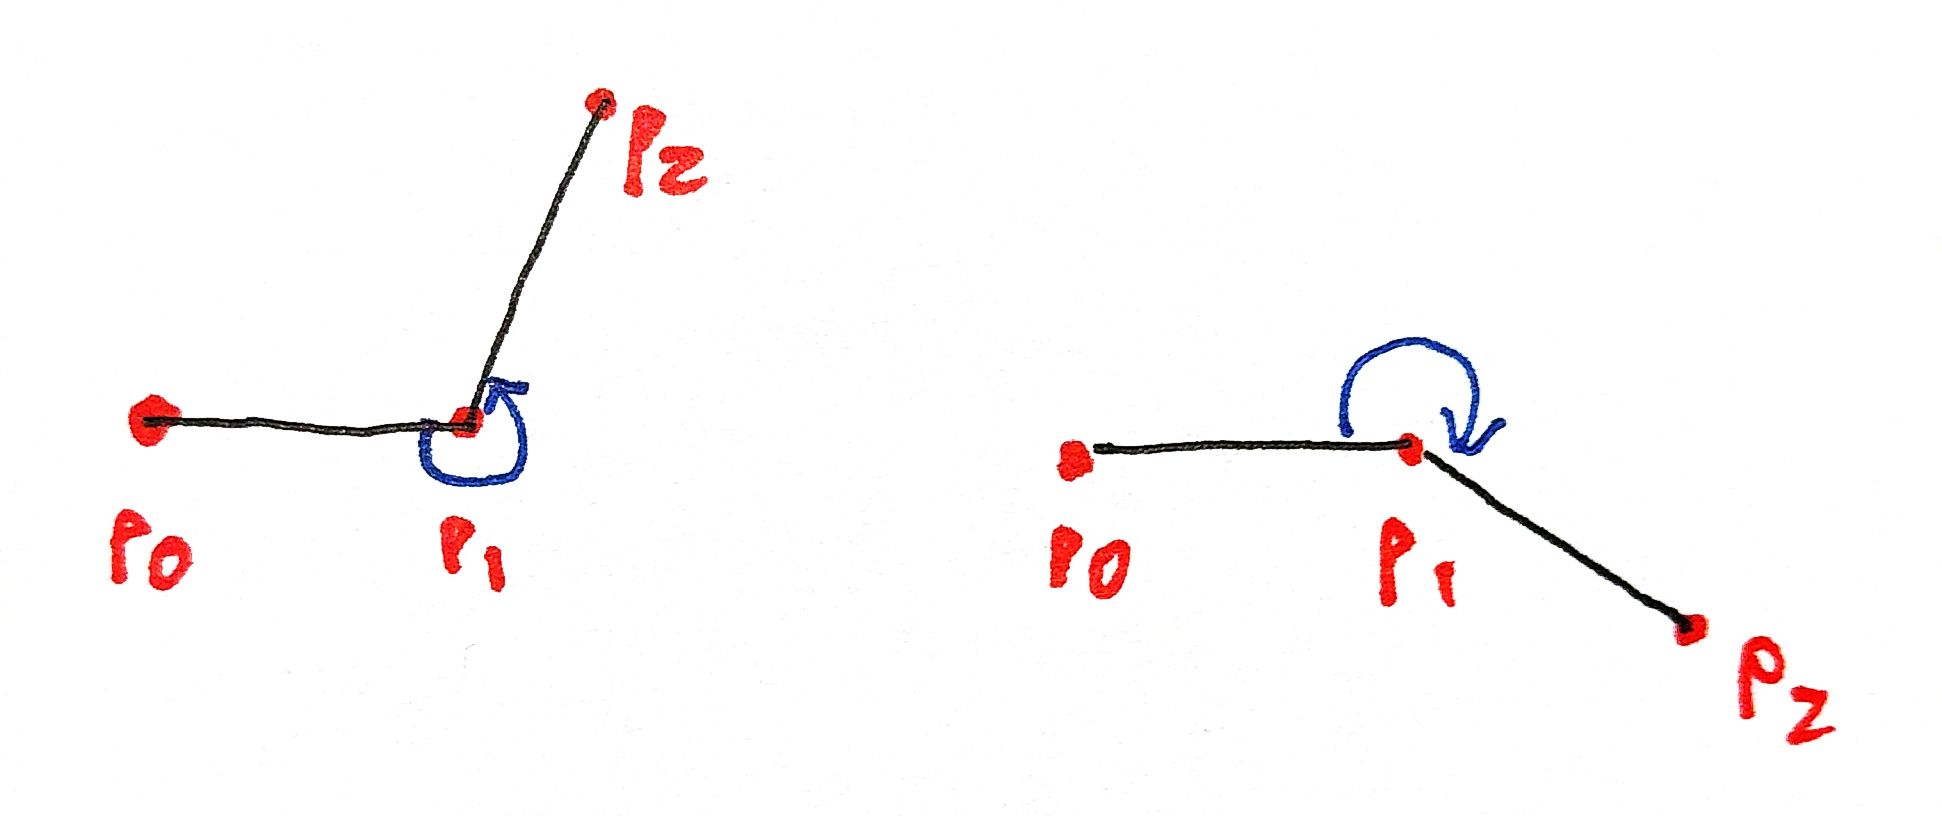
\includegraphics[width=4cm]{segment_lr.jpg} \\

    \vspace{2cm}
    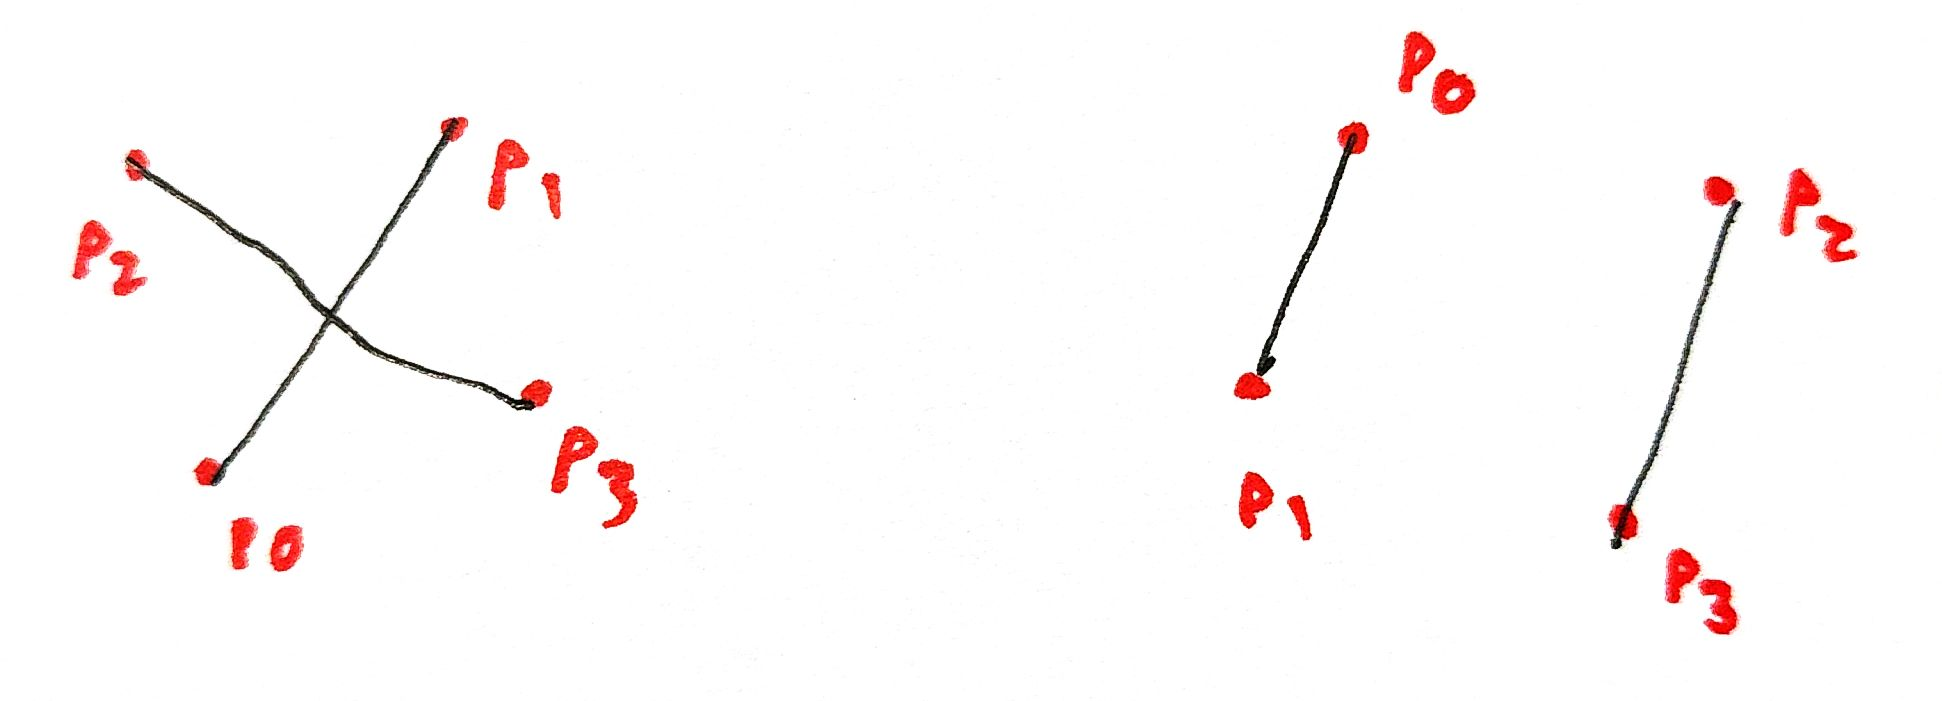
\includegraphics[width=6cm]{segment_intersect.jpg}
  \end{center}
\end{frame}
  
\begin{frame} \frametitle{Degeneracy and Non-Degeneracy Assumptions}
\textbf{degenerate} object: has the proper shape/type, but the values are a
  special case that betrays the spirit of the definition \stanza

\emph{Example:} triangle $\equiv$ three points $(p_1, p_2, p_3)$ \\
degenerate triangle: $p_1=p_2=p_3$, or all points colinear \stanza

  \begin{center}
    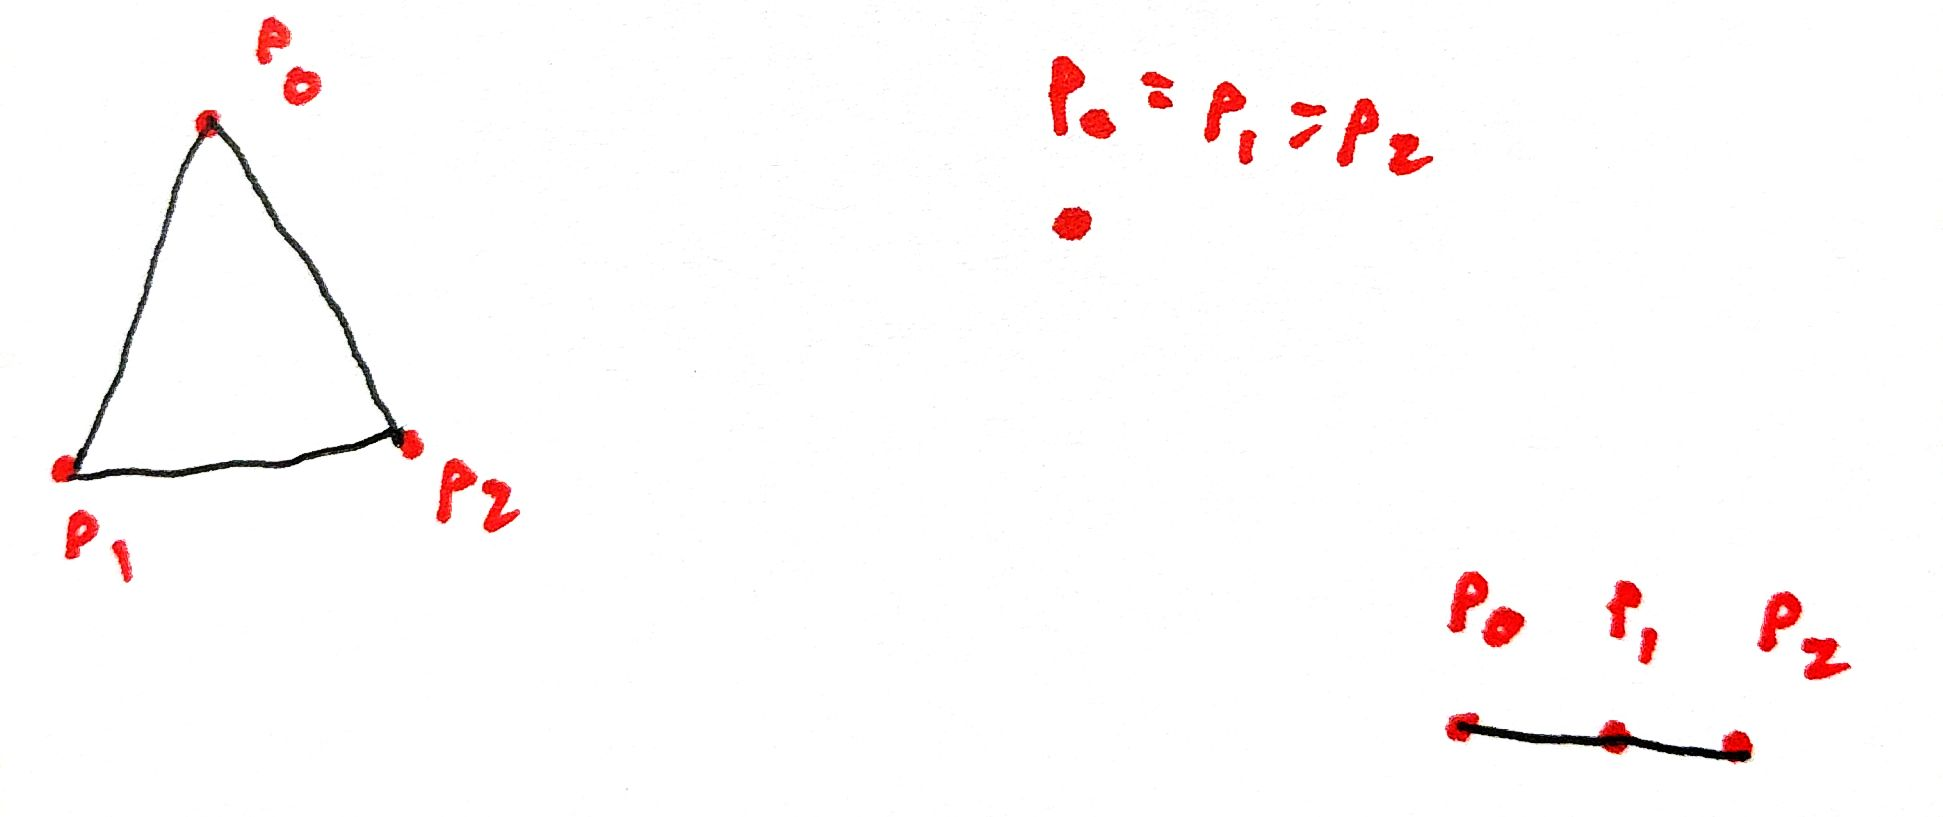
\includegraphics[width=6cm]{degenerate_triangle.jpg}
  \end{center}

\end{frame}

\begin{frame} \frametitle{Non-Degeneracy Assumptions}
\textbf{non-degeneracy assumption}:
\begin{itemize}
  \item constraint that input to a CG algorithm is not degenerate in specific ways
  \item simplifies algorithm design
  \item assume that in practice, some combination of
  \begin{itemize}
    \item degeneracies do not occur
    \item input can be preprocessed to remove degeneracies
    \item implementer can modify algorithm to handle degeneracies
  \end{itemize}
\end{itemize}
\end{frame}

\begin{frame} \frametitle{Sweep Algorithms}
A pattern in CG algorithms:
\begin{itemize}
  \item \emph{line sweep:} envision a line ``sweeping'' through the input
  \item e.g. a vertical line sweeping left-to-right
  \item helps us visualize a 2D situation as a 1D situation that changes over
    time
  \item like duality, doesn't actually change the problem, but might help us
    problem-solve
  \item generalizes to higher dimensions e.g. plane sweep in 3D, hyperplane sweep
    in any dimension
\end{itemize}
\end{frame}

\begin{frame} \frametitle{Sweep Algorithms}
  \begin{center}
    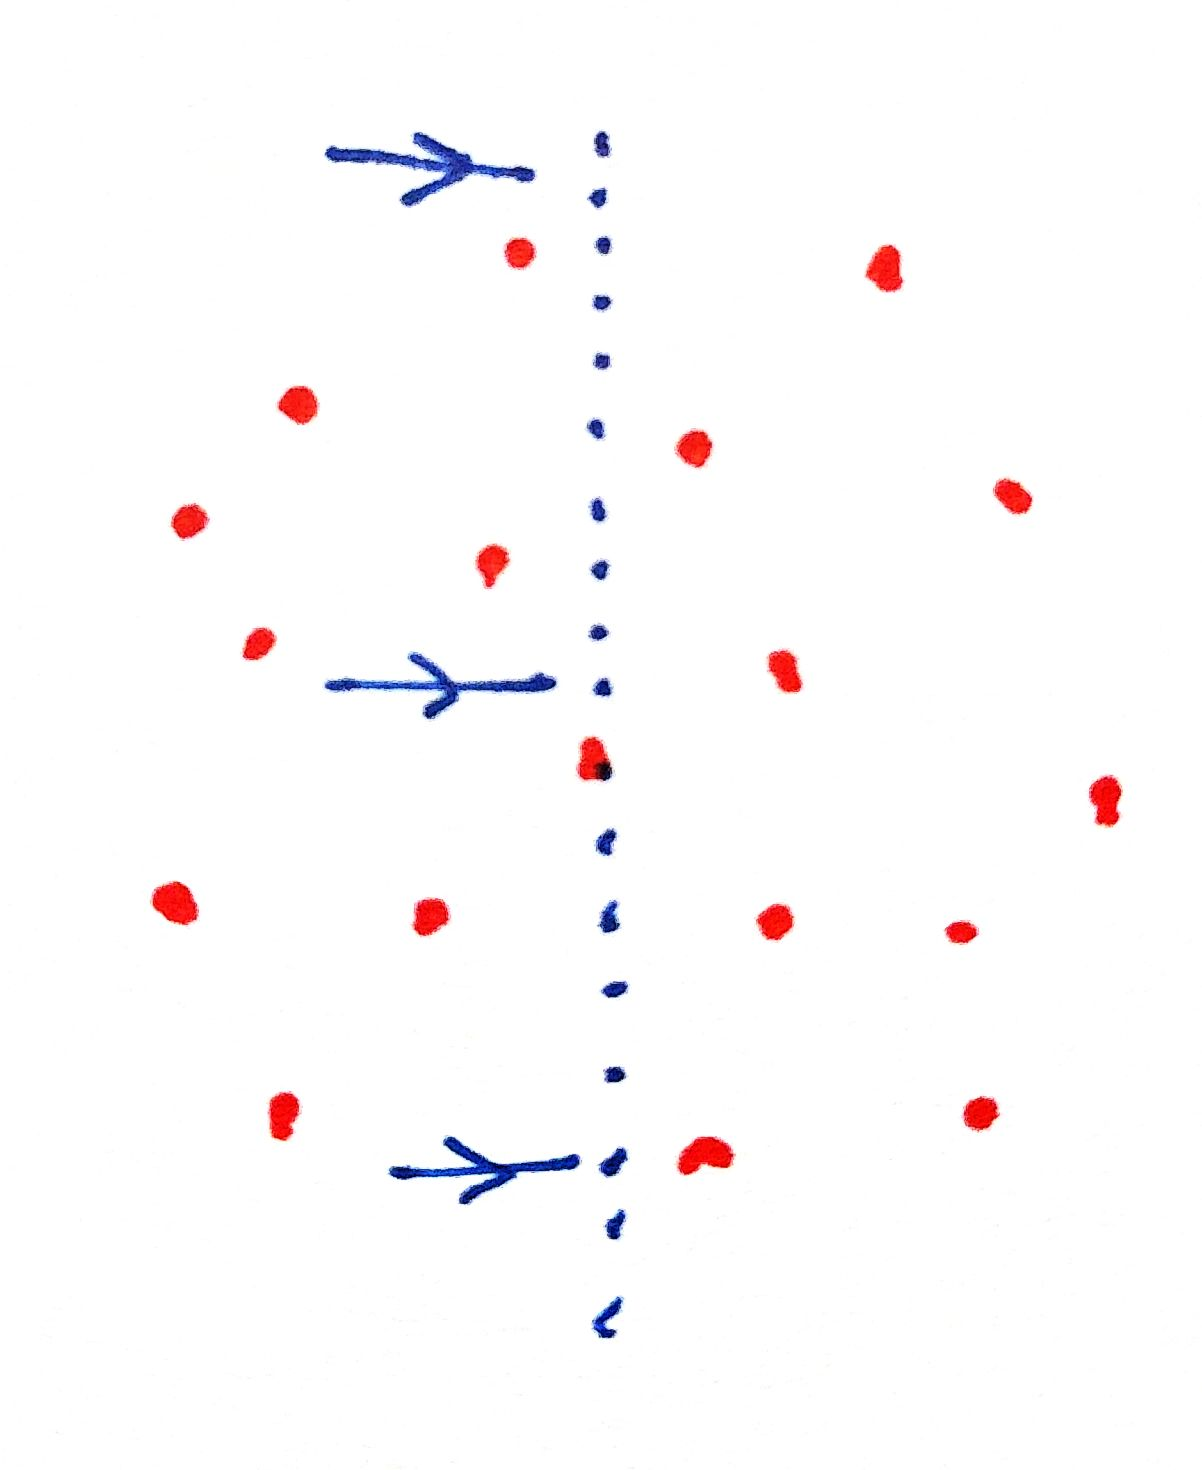
\includegraphics[width=6cm]{line_sweep.jpg}
  \end{center}
\end{frame}

\end{document}
